% Standalone TikZ source for zero_wam_action_channels.png.
% Colors encode decoded value type. The narrow top stripe encodes side.
% A dark stripe means the released metadata does not establish left/right order.
\documentclass[tikz,border=8pt]{standalone}
\usepackage{tikz}
\definecolor{position}{HTML}{63C5DA}
\definecolor{quaternion}{HTML}{B696E6}
\definecolor{joint}{HTML}{F2B65F}
\definecolor{gripper}{HTML}{80CA91}
\definecolor{inactive}{HTML}{E5E7EB}
\definecolor{leftside}{HTML}{2453A6}
\definecolor{rightside}{HTML}{C14472}
\definecolor{unspecified}{HTML}{46505C}

\begin{document}
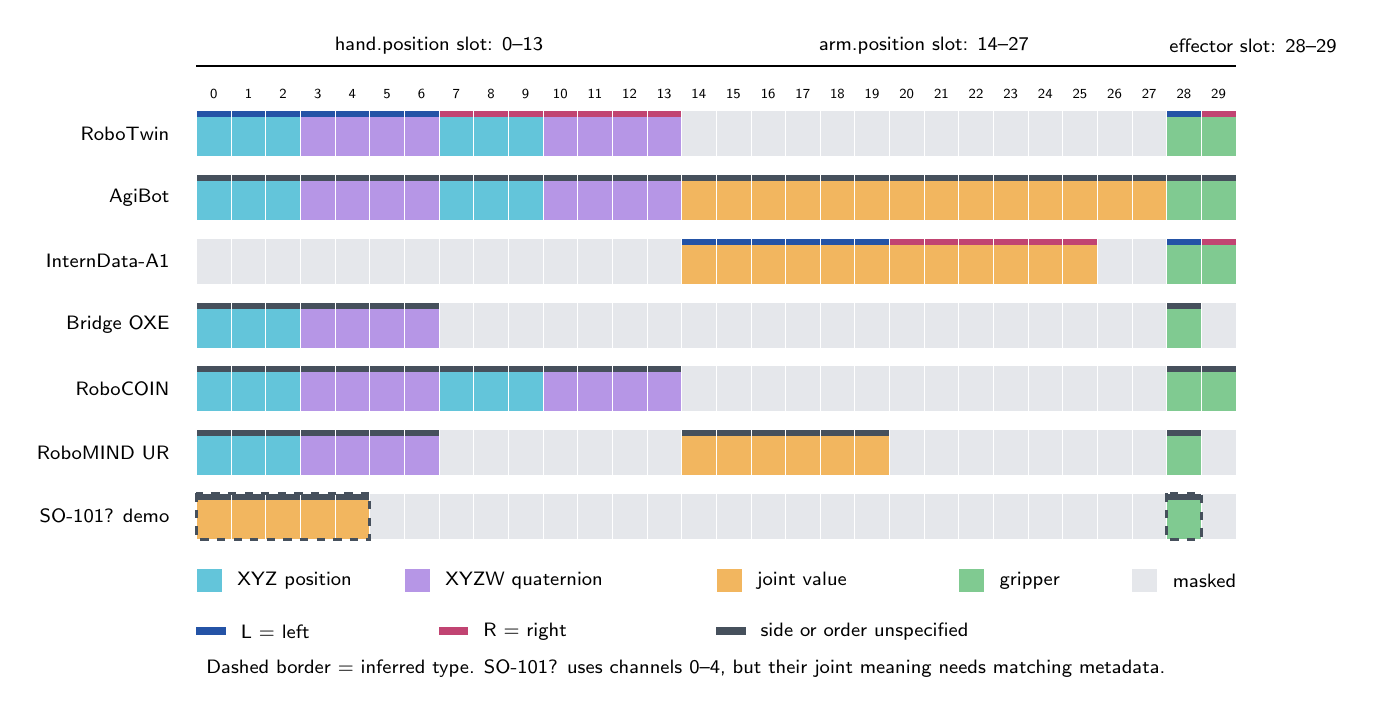
\begin{tikzpicture}[x=0.44cm,y=0.81cm,font=\sffamily\scriptsize]
  % Each channel is one cell. The colored strip above it encodes L/R/unknown.
  \newcommand{\paint}[5]{%
    \foreach \i in {#2,...,#3} {\pgfmathtruncatemacro{\next}{\i+1}%
      \fill[#4] (\i,-#1) rectangle (\next,{-#1-0.72});%
      \fill[#5] (\i,-#1) rectangle (\next,{-#1-0.105});%
      \draw[white,line width=0.2pt] (\i,-#1) rectangle (\next,{-#1-0.72});%
    }%
  }
  \foreach \r in {0,...,6} {\paint{\r}{0}{29}{inactive}{inactive}}

  % RoboTwin: left and right end-effector poses, then left/right grippers.
  \paint{0}{0}{2}{position}{leftside}
  \paint{0}{3}{6}{quaternion}{leftside}
  \paint{0}{7}{9}{position}{rightside}
  \paint{0}{10}{13}{quaternion}{rightside}
  \paint{0}{28}{28}{gripper}{leftside}
  \paint{0}{29}{29}{gripper}{rightside}

  % AgiBot's transform establishes two poses and 14 joints, but does not
  % explicitly label the ordering within those fields as left versus right.
  \paint{1}{0}{2}{position}{unspecified}
  \paint{1}{3}{6}{quaternion}{unspecified}
  \paint{1}{7}{9}{position}{unspecified}
  \paint{1}{10}{13}{quaternion}{unspecified}
  \paint{1}{14}{27}{joint}{unspecified}
  \paint{1}{28}{29}{gripper}{unspecified}

  % InternData-A1 names its left and right joint/gripper origin fields.
  \paint{2}{14}{19}{joint}{leftside}
  \paint{2}{20}{25}{joint}{rightside}
  \paint{2}{28}{28}{gripper}{leftside}
  \paint{2}{29}{29}{gripper}{rightside}

  % Euler-valued source poses become XYZ + XYZW quaternion model channels.
  \paint{3}{0}{2}{position}{unspecified}
  \paint{3}{3}{6}{quaternion}{unspecified}
  \paint{3}{28}{28}{gripper}{unspecified}

  \paint{4}{0}{2}{position}{unspecified}
  \paint{4}{3}{6}{quaternion}{unspecified}
  \paint{4}{7}{9}{position}{unspecified}
  \paint{4}{10}{13}{quaternion}{unspecified}
  \paint{4}{28}{29}{gripper}{unspecified}

  \paint{5}{0}{2}{position}{unspecified}
  \paint{5}{3}{6}{quaternion}{unspecified}
  \paint{5}{14}{19}{joint}{unspecified}
  \paint{5}{28}{28}{gripper}{unspecified}

  % Image-based SO-101 identification; action type is inferred from config.
  \paint{6}{0}{4}{joint}{unspecified}
  \paint{6}{28}{28}{gripper}{unspecified}
  \draw[very thick,dashed,unspecified] (0,-6) rectangle (5,-6.72);
  \draw[very thick,dashed,unspecified] (28,-6) rectangle (29,-6.72);

  \foreach \r/\name in {0/RoboTwin,1/AgiBot,2/InternData-A1,3/Bridge OXE,4/RoboCOIN,5/RoboMIND UR,6/SO-101? demo} {
    \node[anchor=east] at (-0.5,{-\r-0.36}) {\name};
  }

  % Column indices and capacity-block boundaries.
  \foreach \i in {0,...,29} {
    \node[font=\sffamily\tiny] at ({\i+0.5},0.26) {\i};
  }
  \draw[thick] (0,0.70)--(14,0.70);
  \draw[thick] (14,0.70)--(28,0.70);
  \draw[thick] (28,0.70)--(30,0.70);
  \node at (7,1.02) {hand.position slot: 0--13};
  \node at (21,1.02) {arm.position slot: 14--27};
  \node[anchor=west] at (27.8,1.02) {effector slot: 28--29};

  % Legends: fill = type; narrow top stripe = side.
  \foreach \x/\tone/\name in {0/position/XYZ position,6/quaternion/XYZW quaternion,15/joint/joint value,22/gripper/gripper,27/inactive/masked} {
    \fill[\tone] (\x,-7.55) rectangle ({\x+0.75},-7.18);
    \draw[white] (\x,-7.55) rectangle ({\x+0.75},-7.18);
    \node[anchor=west] at ({\x+0.9},-7.37) {\name};
  }
  \foreach \x/\tone/\name in {0/leftside/L = left,7/rightside/R = right,15/unspecified/side or order unspecified} {
    \fill[\tone] (\x,-8.22) rectangle ({\x+0.85},-8.10);
    \node[anchor=west] at ({\x+1.0},-8.17) {\name};
  }
  \node[anchor=west] at (0,-8.75) {Dashed border = inferred type. SO-101? uses channels 0--4, but their joint meaning needs matching metadata.};
\end{tikzpicture}
\end{document}
